\subsection{Efficiency Evaluation}
\label{sec:results_eff}
%
In this section, we evaluated the efficiency of our prioritizing algorithms in terms of the overhead added to the automatic recommendation engine RtSEngine.
%
We report the overhead as the execution time averaged over 5 runs.
%
%the costs of executing the proposed algorithms and gains of applying 
%	the algorithms. 
%
Similar to previous experiments,  we vary $K$ and $R$, and compare with the actual execution of SeeDB engine as a baseline.
%
 %All the experiments were repeated 5 times and the measurements were averaged. We begin by presenting a summary of our experimental
%findings and then dive into performance results for individual optimizations.
%
%we compared the executions costs of the algorithms added to SeeDB with the original  baseline of SeeDB to identify the improvements in the performance. 
%

As shown in Figure \ref{fig:fig33}, the total execution time of the algorithms are compared with the original SeeDB baseline. 
%
%The figure shows that improvements in the SeeDB performance with different $R$ values to find Top-25 $(K = 25)$ views. 
%
As shown, the improvements in the performance by using the proposed algorithms are significant when compared with the baseline. 
%
Furthermore, the execution time of our proposed algorithms increases linearly with $R$.
%
%\mas{what happens after 120? do the other two also exceed SeeDB?}
\begin{figure}[t]
   \centering
%\end{figure}
  \begin{subfigure}[b]{0.42\textwidth}
    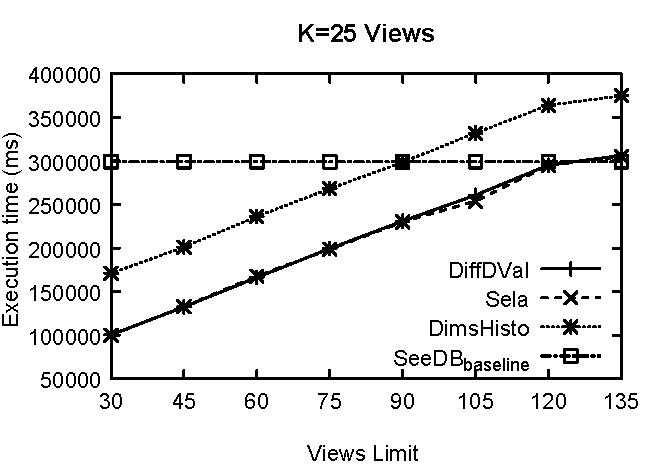
\includegraphics[width=\textwidth]{33.pdf}
    \caption{Execution time while varying $R$}
    \label{fig:fig33}
  \end{subfigure}
  %
  \begin{subfigure}[b]{0.42\textwidth}
    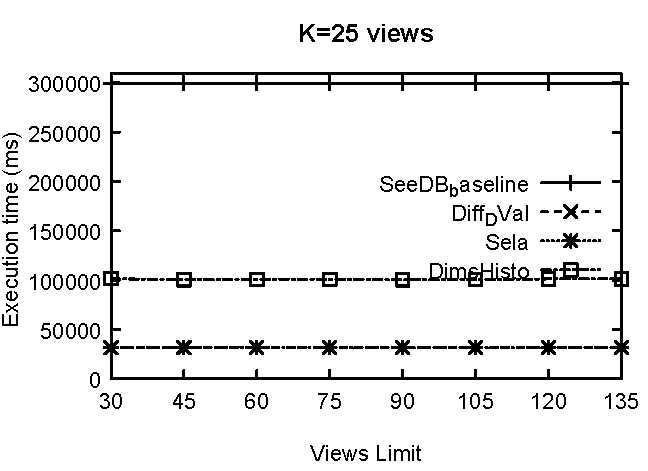
\includegraphics[width=\textwidth]{34.pdf}
    \caption{Average overhead}
    \label{fig:fig34}
  \end{subfigure}
  \caption{Algorithms performance while varying $R$}
\end{figure}

%\mas{very confusing plot! what are the different components? and what are they stacked on top of each other?}
The execution time shown in Figure \ref{fig:fig34} is the extra overhead needed by our proposed algorithms.
%
As shown, the average overhead is almost stable along different $R$ values.
%
This is because our algorithms evaluate a fixed set of dimension attributes every time, regardless of the value of $R$. 
%
The high cost of $DimsHisto$ is due to its nature: it processes a number of queries to create histograms for computing the distance among them.

\begin{figure}[t]
   \centering
%\end{figure}
  \begin{subfigure}[b]{0.42\textwidth}
    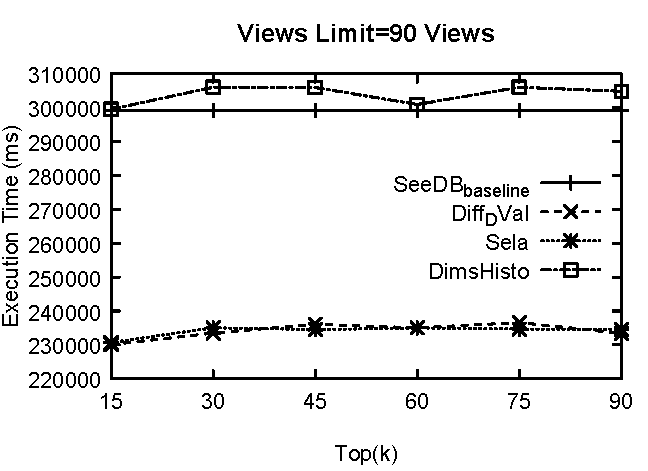
\includegraphics[width=\textwidth]{31.pdf}
    \caption{Total execution time while varying $K$ and $R=90$}
    \label{fig:fig31a}
  \end{subfigure}
  %
  \begin{subfigure}[b]{0.42\textwidth}
    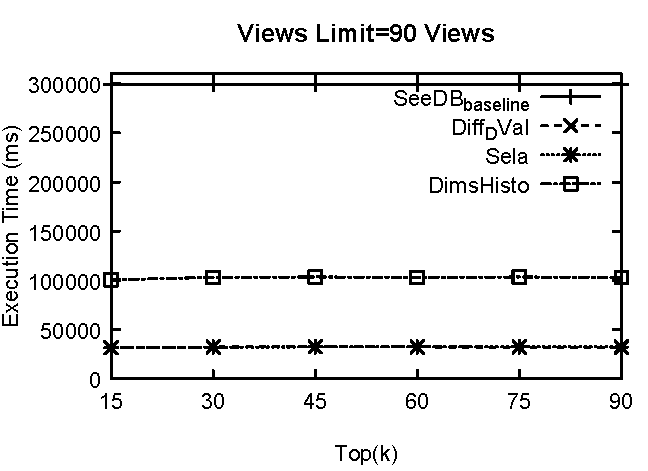
\includegraphics[width=\textwidth]{32.pdf}
    \caption{Average overhead while varying $K$ and $R=90$}
    \label{fig:fig32}
  \end{subfigure}
  \caption{Algorithms performance on varying $K$}
\end{figure}

The following experiments discuss the efficiency of the proposed algorithms along different $K$ values.
%
As shown in Figure \ref{fig:fig31a}, the proposed algorithms show improvements in the execution. 
%
More than \%40 when compared with the SeeDB baseline execution time. 
%
As shown above, $DimsHisto$ shows the highest cost among the algorithms $Sela$ and $Diff DVal$. 
%

Figure \ref{fig:fig32} shows the average overhead of the algorithms while varying $K$.
%
The overhead is almost constant while increasing $K$.
%
This is because the space limit $R$ is constant too.